%%%%%%%%%%%%%%%%%%%%%%%%%%%
\chapter {Background and Related Work}
\label{RW}
%%%%%%%%%%%%%%%%%%%%%%%%%%%
\section{ Mobile Ad hoc networks}
\noindent ``Ad-hoc networks are infrastructure-less and cooperation-based networks which means that the network topologies must be decided by the network sensors themselves'' \cite {C14}. In other words, the major feature of ad-hoc networks is that they have no infrastructure.

The Mobile Ad hoc network (MANET), also called the Wireless Ad-hoc Network (WANET), is a decentralized type of wireless network, and there is no~pre-existing infrastructure managing the network, neither. In the MANET, because users move independently, the topology change frequently. Without the help of infrastructure, users can only communicate when they encounter each other. In other words, users communicate only if they are covered by each other's communication range. Because of the previous features, the MANET can be viewed as a kind of delay-tolerant network (DTN) which lacks continuous network connectivity. Then MANET can hardly establish instantaneous end-to-end paths, which compel the routing protocols in MANET to use a characteristic strategy ``store-and-forward''. Uses forward messages when they encounter others, or they just store messages, as shown in Figure 2.1. The user A has a message to the user C, so he sends the message to the user B when they encounter each other. The user B stores the message and moves, until he meets the user C. When the user B and the user C make contact, the user B sends the message to the user C, so that the message is delivered. It is obvious that whether the message can be delivered depends on the movement of users. If the user B never meet the user A or the user C, the message must be dropped after the timeout. The delivery process might be low success ratio and time-consuming.

\begin{figure} [H]
  \centering 
  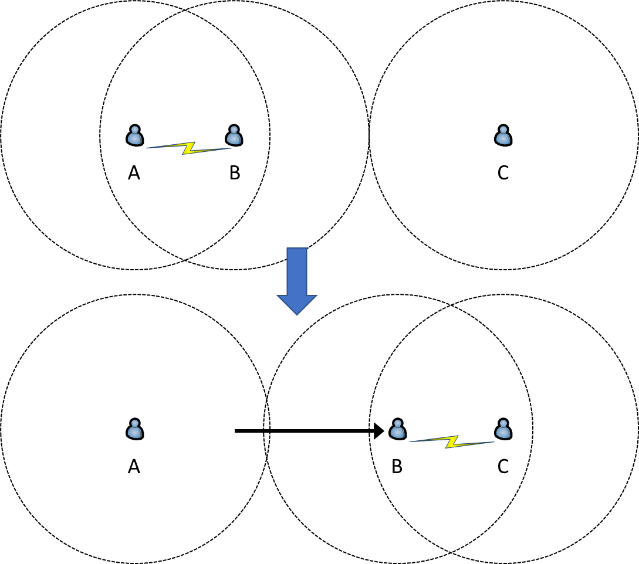
\includegraphics[width=4.0in]{figures/FIG_MANET.png}
  \caption{MANET} 
  \label{fig:MANET} %% label for entire figure 
\end{figure}

\section{ Delay Tolerant Network}

\noindent Regular networks, e.g. Internet, always have end-to-end paths. As shown in Figure 2.2, the node S and the node D are connected by A, B, and C. Their maximum round-trip time is not excessive, and their drop probability is also small. Comparing to the regular network, there is a class of challenged networks \cite {C1} which lacks end-to-end path and suffering from high latency and long queuing times. As shown in Figure 2.3, when the node B is not working, there is no connection between the node A and the node C, so that extensive latency is inevitable if the source S sends a message to the destination D.

\begin{figure} [H]
  \centering 
  \subfigure[Regular Network]{ 
    \label{fig:comparison_RN_DTN:a} %% label for first subfigure 
    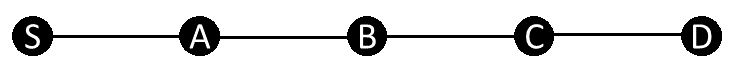
\includegraphics[width=4.0in]{figures/FIG_Regular_Network.png}} 
  \hspace{1in} 
  \subfigure[DTN]{ 
    \label{fig:comparison_RN_DTN:b} %% label for second subfigure 
    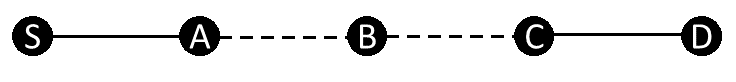
\includegraphics[width=4.0in]{figures/FIG_DTN.png}}
  \caption{The comparison between regular networks and DTNs} 
  \label{fig:comparison_RN_DTN} %% label for entire figure 
\end{figure}

\noindent Since the challenged networks have significant differences with the regular networks, researchers introduce a new architecture Delay Tolerant Network (DTN) to deal with the unique features in the challenged works. Terrestrial Mobile Networks, Exotic Media Networks, Military Ad-Hoc Networks and Sensor/Actuator Networks are typical DTNs.


\subsection{ Spray and Wait}

\noindent The Spray and Wait is a known protocol for DTNs. Although it is not as efficient as protocols on internet, it works in DTNs. A message is initialized with several copies, a part of which are given to others when users encounter each other. Users keep forwarding copies until they each have only one copy of the message. When a user carrying at least one copy of the message encounters the destination, he gives all his copies to the destination to finish the delivery. The Binary Spray and Wait (BSW) is an optimized version of the Spray and Wait, which is also used in our protocols. The user who creates the message also makes several copies of that message. He gives half of the copies the user whom he encounters so that both he and the other user have a half of the copies. The users who get copies of the message continue to give a half of copies holding by them to others until they have only one copy. The remained one copy is given to the destination only.

\subsection{ Other Protocols}


\subsubsection{ Direct Contact Scheme}

\noindent The simplest strategy for DTN is that the source holds the message until he meets the destination, which is called the direct contact scheme. So, a direct path between the source and the destination is necessary for a success delivery. It is possible that the source never comes in contact with the destination so that message is not delivered. 


\subsubsection{ Replica Based Protocols}

\noindent The replica based protocols work by making several replicas of the message so that users can retransmit them upon connection establishment. The former BSW is also a kind of replica based protocols. Comparing to the direct contact scheme, the replica based protocols make it more possible for messages to be delivered. But they require more resources than the direct contact scheme because they need more memory to store the replicas. Therefore, making a reasonable decision for the message replication and dropping is the key to these kinds of protocols.


\subsubsection{  Knowledge-Based Protocols}

\noindent Different from the former replica protocols which require no knowledge about the topology of the network, the users in knowledge-based protocols try to evaluate their own view of the topology of the network so that they can make better forwarding decisions. However, the topology changes so frequently that it is hard for users to have an accurate topology.


\subsubsection{ Coding Based Protocols}

\noindent Authors in \cite {C12} and \cite {C13} make the approach by introducing coding techniques into routing protocols. Instead of making a few replicas, coding based protocols encrypts data to make a large number of message blocks. If the destination receives a part of the blocks, he can decrypt the message.

\section{ Location-Based Services}

\noindent The Location-Based Services (LBS) use users' location information to provide services, which is shown in Figure 2.4. Your smartphone can detect your coordinate and send it to LBS application server which is responsible to provide service based on the coordinate. The point of interest and the location advertisement are familiar instances of LBS. The LBS providers collect users' location information to provide services, which makes LBS providers a significant target of attackers. When attackers access the databases of the LBS providers, they can learn all sensitive information in the servers. So, the LBS providers should be viewed as semi-trusted, which might expose information in front of vicious attackers.

Users face risks of information breach when they access a semi-trusted LBS provider because anyone who has access to data in LBSs is able to steal and misuse LBS users' location-privacy. Considering that LBSs rely on location-aware computing, it is unavoidable to leak users' location from LBSs. Therefore, balancing ?these two competing aims of location privacy and location awareness? \cite {C20} is always a challenge.

\begin{figure} [H]
  \centering 
  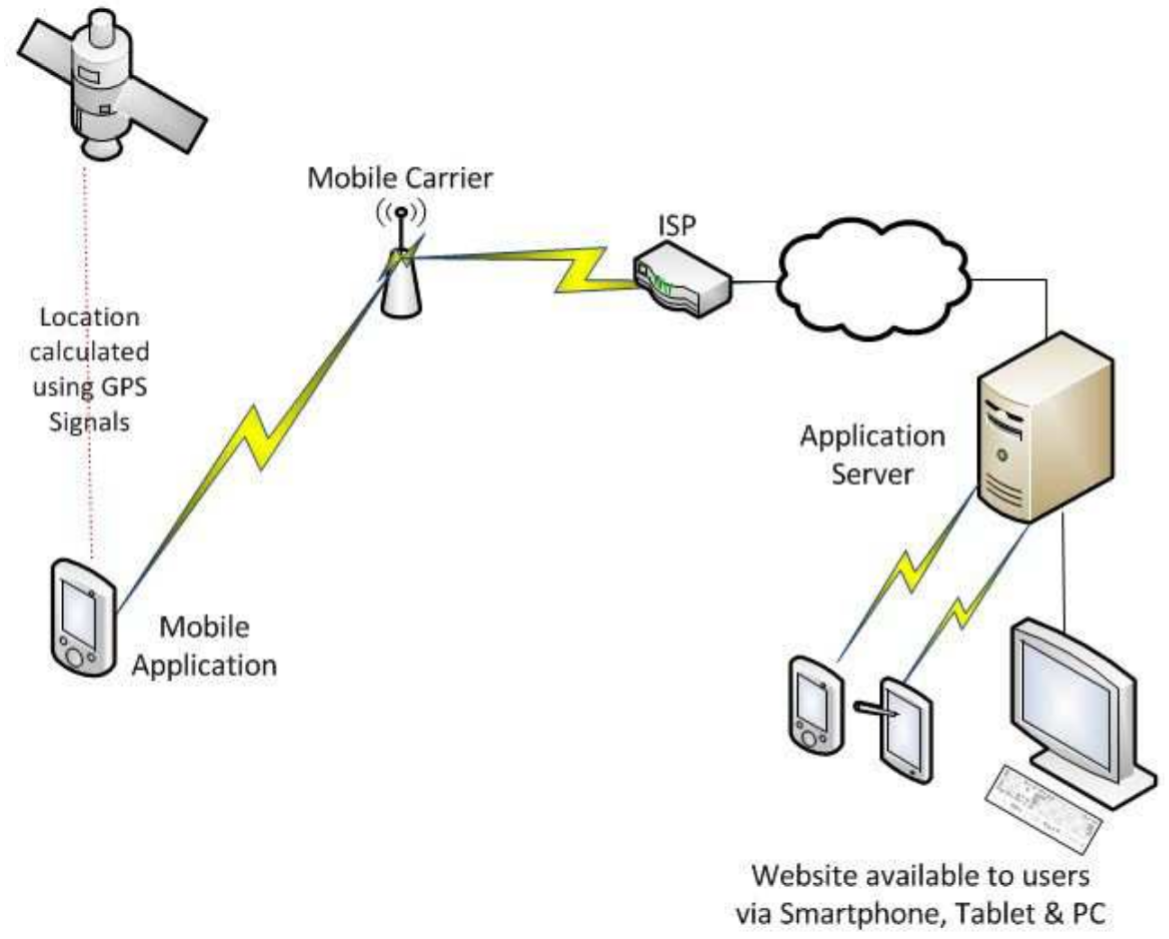
\includegraphics[width=4.0in]{figures/FIG_LBS_11.png}
  \caption{LBS \cite {C11}} 
  \label{fig:LBS} %% label for entire figure 
\end{figure}

\section{ Social Network}

\noindent Social networks which contains social interactions and personal relationships are used in location-privacy protection so that users can determine who is trustful. In \cite {C30}, the relationship of a pair of people (e.g., a user $i$ and a user $j$) is described as a pair of directed relationship strengths. The directed relationship strength from the user $i$ to the user $j$ can be denoted by ${RS}^{ij}$. We should notice that ${RS}^{ij}$ might be unequal to ${RS}^{ji}$, because the user $i$ might like the user $j$ so much while the user $j$ just views the user $i$ as an acquaintance. Based on the relationship strength, researcher can estimate the relational tie between two people and predict whether they are friends or strangers. 

The relationship strength is compared with a threshold, if the relationship strength is higher than the threshold the two people are friends, or they are strangers. In the protocols we mentioned in the thesis, researchers always assume that friends are trustful. That is reasonable because you might feel more secure when your friends forward your message instead of a stranger. 


\section{ Location-privacy protocols}

\noindent The basic idea of most location-privacy protocols is hiding the original requester behind a set of users so that attackers can hardly infer the identity of the original requester. In other words, when a user sends a query, his identity cannot be inferred based on the information in the query easily. For example, the original requester can use a pseudonym instead of his own name or use an obfuscated location to send his queries, so that attackers cannot tell the different between the queries and a set of other users' queries. 

The location-privacy protocols are considered as centralized and distributed ones based on whether they require any infrastructure. 


\subsection{ Centralized Protocols}

\noindent Centralized Protocols always need some infrastructure to serve for the obfuscation process. The infrastructure could be any equipment which act as anonymization servers. When users want to send a query to the LBS server, he sends the query to the anonymization server. The anonymization server changes the identity and the location in the query, which is called anonymization or obfuscation. Then the anonymization server forwards the modified query to the LBS server, so that the attacker who attacks the LBS server can hardly learn the identity of the original requester. The LBS server can send the reply message to the anonymization server which is responsible and able to forward the reply message back to the original requester. In this way, the original requester gets the information he needs, while avoiding from being located by attackers.

The advantage of the centralized protocols is that the anonymization server has more resources and information than users in the network, which enable the server to achieve better anonymization performance and provide sufficient protection for users. For example, if the anonymization server knows locations of all users in the network, it can modify the location and identity in the queries to the most suitable, with which the LBS server can provide acceptable results while the original requester is not exposed.

There are three major defects of this kind of protocol. 1. It is hard to deploy infrastructure in some area; 2. Since the anonymization server knows users' location, it is also a risk for users.


\subsubsection{ Single Server}

\noindent Authors in \cite {C15} uses a central anonymity server through which the mobile users can send queries to external services. To make the communication between users and the central anonymity server trustful, users set up an encrypted connection with the anonymity server at the beginning. Users sends their encrypted queries to the anonymity server, so that the anonymity server is the only one who can learn the information in the query. The anonymity server decrypts the queries and uses a cloaking algorithm to perturb the position information in the queries. Then the anonymity server sends the modified queries to external services (e.g. LBS). This is a typical centralized protocol, which can reduce the re-identification risk for users. Its defect is that a continuous connection to the server is necessary for each user, which is hard to achieve in a sparse DTN. We cannot image that a MANET user can have a stable connection with a central anonymity server, neither.

In \cite {C23}, researchers employ a matchmaker which is used to match users and advertisements, then users can achieve anonymization of their identities and locations from the matchmaker. The system architecture in \cite {C23} is similar to the former \cite {C}, while authors in \cite {C23} just focus on the advertisement service instead of the ?external services? in \cite {C23}. The role of matchmaker is matching users and advertisements. Although the functions of the matchmaker in \cite {C23} and the central anonymity server in \cite {C15} are different, the intermediate trusted three-party servers (i.e., the matchmaker and the central anonymity server) separate users and the application server (e.g., an advertisement server, LBS server and so on). The architecture in \cite {C23} does not require an encryption process so that attackers can learn the information in the queries. Although a plenty of queries arrive the matchmaker in a short time from different users also help the matchmaker mix the queries so that attackers can hardly trace the query, the burden of the users who are near the matchmaker is heavy.

In the work in \cite {C24}, researchers use ?a trusted, third-party location anonymization engine (LAE) that acts as a middle layer between mobile users and LBS providers? \cite {C24}, so that exact locations and requests from clients are replaced by a location anonymization engine before they arrive at LBS providers. Therefore, we learn that the structure of this kind of algorithms is almost like Figure 2.5. A trusted server is placed between users and the application server, which hides users' information and offers sufficient information for the application servers to provide acceptable services. 

\begin{figure} [H]
  \centering 
  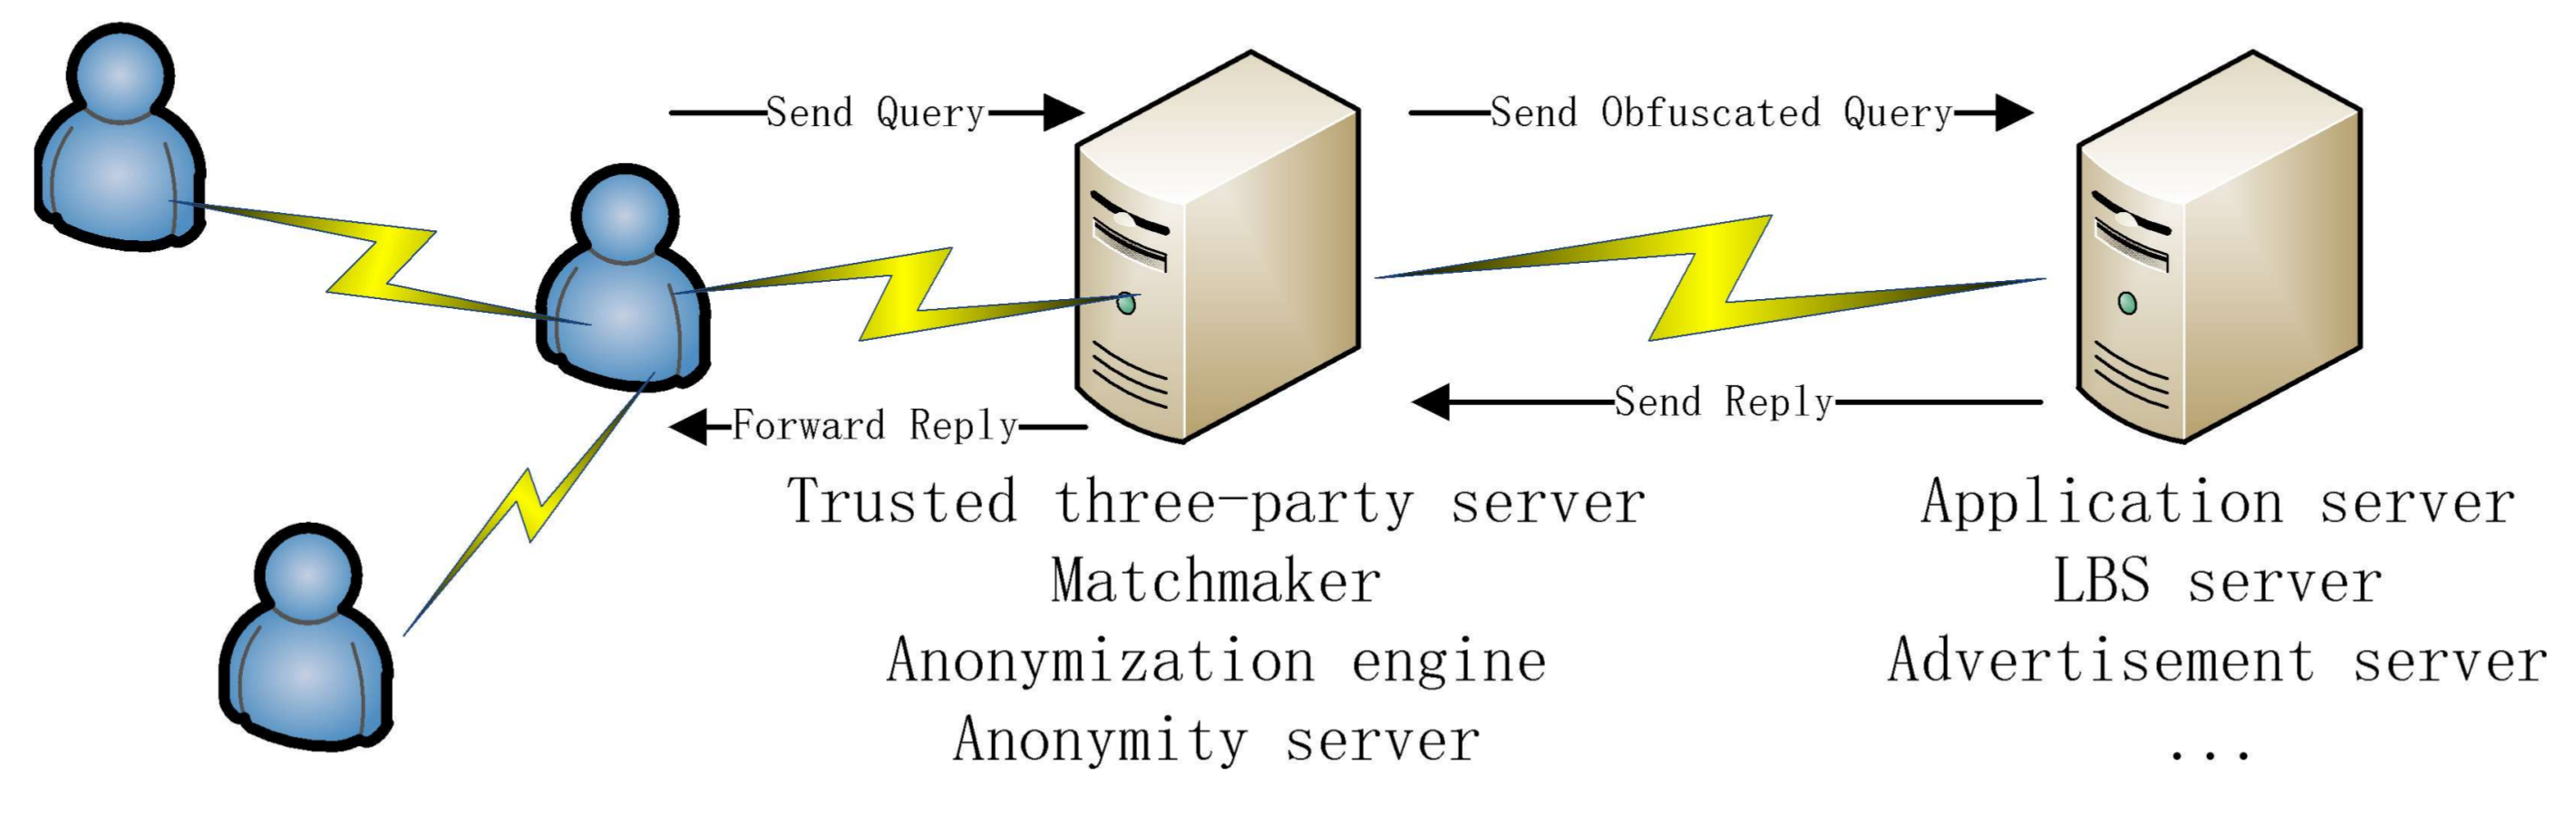
\includegraphics[width=4.0in]{figures/Fig_Single_Ano_Ser.png}
  \caption{Single Anonymization Server} 
  \label{fig:SingleAnoymizationServer} %% label for entire figure 
\end{figure}

\subsubsection{ Multiple Servers}

\noindent The above protocols always use a single anonymization server, while there are also other protocols which need more infrastructures. 

Authors in \cite {C25} propose a protocol, called Social-based PRivacy-preserving packet forwardING (SPRING), for vehicular delay tolerant network. In their work, they employ Roadside Units (RSUs), which are a type of equipment deployed along the roadside, to assist the packet forwarding and achieve conditional privacy preservation. These RSUs are located at high social intersections, so that vehicles which pass by the RSUs send their messages to the RSUs. The RSUs have sufficient resource so that they can hold the messages for a long time, which decrease the probability that the messages are dropped. The messages are forwarded to proper next-hop vehicles when the vehicles pass by the RSUs. Since messages are hold by the RSUs for a period, attackers can hardly trace messages. Besides, a large number of vehicles send many packets to these RSUs, which enables the RSUs to serve as mix servers. The advantage of SPRING is that it improves the delivery success ratio and privacy-protection performance. However, deploying the RSUs is not always feasible.

Another example is the work in \cite {C26}. Researchers use sensor nodes which are scattered throughout the network to provide anonymized locations for users, as shown in Figure 2.6. The whole system area is partitioned into a set of aggregate locations by the sensor nodes, where there are at least $k$ persons. To provide better location-based services, they minimize the areas of aggregate locations. When a user sends a query to the LBS, he uses the location of the sensor nodes which he belongs to, so that attackers cannot tell the difference between the requester and the other $k-1$ users in that aggregate location. This is a typical k anonymity algorithm, while its disadvantage is that it is difficult to deploy the sensor nodes in real-world. Besides, the mix servers and sensor nodes might be more prominent targets than LBS providers.

\begin{figure} [H]
  \centering 
  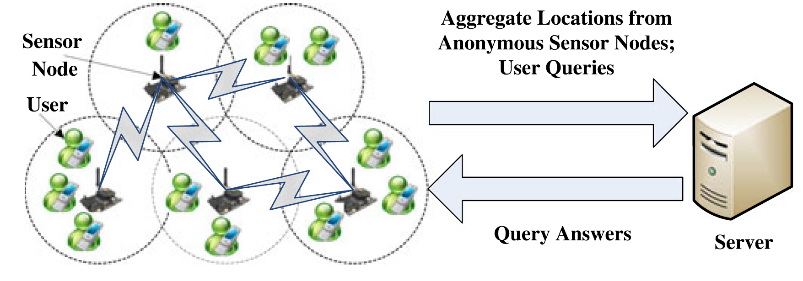
\includegraphics[width=4.0in]{figures/FIG_REAL_26.png}
  \caption{REAL \cite{C25}} 
  \label{fig:REAL} %% label for entire figure 
\end{figure}

\subsection{ Distributed Protocols}

\noindent Although centralized protocols also have good performance in their delivery success ratio and privacy-protection in their own field, the MANET is a network without infrastructure. In general, it is not allowed that deploy any infrastructure for MANET. Distributed protocols are organized by users independently so that they are more proper for applications in MANET. A problem for a distributed protocol it that whether a user can trust another one. Authors in \cite {C16}, \cite {C17} and \cite {C18} introduce the social tie to determine whether a user is trustful.

In the distributed social based location privacy protocol (SLPD) \cite {C16}, authors import 2 concepts: the obfuscation phase and the free phase. A query from an original requester is initialed as the obfuscation phase, then it must be transmitted between friends for $k$ times. For example, the original requester sends the query to one of his friend in one hop, then the friend forwards the query to another friend. We call these friends the agents. That process repeats for exact $k$ times. When the $k^{th}$ friend get the query, he switches the query to the free phase and replaces the sender identity with his own identity, then sends the query to the destination (e.g., LBS) with any DTN protocol. The LBS sends the reply to the friends and they are responsible to forward the message to the original requester. 

In this way, attackers can only learn the identity of the last friend instead of the original requester. Since each user who knows the identity of the original requester is the original requester's friend who are assumed trustful, there are no attackers among these agents. Therefore, attackers can hardly learn the identity of the original requester.

The disadvantage of the protocol is that it is hard to encounter a friend in the network, which decreases the success ratio of delivering queries. The how to improve the success ratio is a key of these protocols.

In Hybrid and Social-aware Location-Privacy in Opportunistic mobile social networks (HSLPO) \cite {C17}, authors try to improve the delivery performance by using a stochastic model which uses a Markov model for location predication. The major process is similar with SLPD, but an agent can forward the query a user who is not a friend of the original requester if the user has more chance to deliver the query and a trust value larger than a threshold. In other words, an agent continuously searching his surrounding to find the original requester's friends. If the agent cannot find the original requester's friend but his own friend, he checks whether his friend has more chance to deliver the query than him using the Markov model. If his friend is more proper for forwarding, he sends the query to his friend. The performance of HSLPO depends on the Markov model, that is, whether it can predict users' movement accurately. In our real-world, people's movement model is more complicated than that in experiment.

Another protocol, called Location Privacy-Aware Forwarding (LPAF) \cite {C18}, also attempt to improve the performance of the SLPD. The LPAF and the SLPD are similar, while the LPAF just add more friends to the protocol. When an agent cannot find a close friend (i.e., their trust value is high), he will try to find other general friends (i.e., their trust values is lower than the close friends). That might be a safety tradeoff, because some ineligible users in SLPD are chosen as friends based on the additional standards imported by LPAF.

In fact, both the HSLPO and LPAF cannot solve the problem in finding friends. Although we use the friends of friends or set the threshold for friends lower, there are only a few users can be chosen as agents. In LPAF, the identity of the requester is even exposed in front of someone who are not very trustful. 




















